%#!platex resume.tex; dvipdfmx resume.dvi
\documentclass{resume}
%\usepackage{amssymb,amsmath}
%\usepackage{listings,jvlisting}
%\usepackage{multicol}
%\usepackage[hyphens]{url}
%\usepackage{graphicx}
%\usepackage[dvipdfmx]{graphicx}
%\usepackage[dvipdfmx]{color}
%\usepackage{xcolor}
%\usepackage{here}
%\usepackage{mathtools}
%\usepackage{stmaryrd}
%\usepackage[dvipsnames]{xcolor}
\usepackage{graphicx}
%\usepackage[dvipdfmx]{graphicx}
\usepackage[dvipdfmx]{color}
\usepackage{float}
\usepackage{listings}
\usepackage{jvlisting} %日本語のコメントアウトをする場合jvlisting(もしくはjlisting)が必要
\usepackage{amsmath}
\usepackage{mathtools}
\usepackage{stmaryrd} % \llparenthesis & rrparenthesis
\usepackage[dvipsnames]{xcolor}
\usepackage[hyphens]{url}
\lstset{
  basicstyle={\ttfamily},
  identifierstyle={\small},
  commentstyle={\small\itshape},
  keywordstyle={\small\bfseries\color{magenta}}, % キーワードの色を青に設定
  ndkeywordstyle={\color{blue}},
  stringstyle={\small\ttfamily\color{green}}, % 文字列の色を緑に設定
  frame={tb},
  breaklines=true,
  columns=[l]{fullflexible},
  numbers=left,
  xrightmargin=0zw,
  xleftmargin=0zw,
  numberstyle={\scriptsize},
  stepnumber=1,
  numbersep=1zw,
  lineskip=-0.5ex,
  keywords={def,for,if,elif,else,return}, 
  ndkeywords={com},% 追加のキーワードを指定
  moredelim=**[is][\color{red}]{pp}{pp} % 特定の要素を赤に設定
}
%\lstset{
%  basicstyle={\ttfamily},
%  identifierstyle={\small},
%  commentstyle={\smallitshape},
%  keywordstyle={\small\bfseries},
%  ndkeywordstyle={\small},
%  stringstyle={\small\ttfamily},
%  frame={tb},
%  breaklines=true,
%  columns=[l]{fullflexible},
%  numbers=left,
%  xrightmargin=0zw,
%  xleftmargin=0zw,
%  numberstyle={\scriptsize},
%  stepnumber=1,
%  numbersep=0.5zw,
%  lineskip=-0.8ex
%}

\renewcommand{\lstlistingname}{Code}
%%%%%%%%%%%%%%%%%%%%%%%%%%%%%%%%%%%%%%%%%%%%%%%%%%
%%% ヘッダ設定
\所属{岐阜大学大学院 自然科学技術研究科 知能理工学専攻}
\研究室{草刈研究室}
\氏名{恩田晴登}
\題目{Pythonの静的型検査器を活用した\\コレオグラフィックプログラミング言語の実装}

%%%%%%%%%%%%%%%%%%%%%%%%%%%%%%%%%%%%%%%%%%%%%%%%%%
%%% ユーザ定義
\renewcommand{\lstlistingname}{code}
\newcommand{\projection}[2]{{\color{cyan}\llparenthesis}#1{\color{cyan}\rrparenthesis^#2}}
\newcommand{\mblue}[1]{\textbf{\textsf{\color{MidnightBlue}#1}}}
\newcommand{\cyan}[1]{\color{cyan}#1}
\newcommand{\gr}[1]{\color{ForestGreen}#1}
\newcommand{\nl}[1]{{\color{red}{\llbracket}}#1{\color{red}{\rrbracket}}} % Normalizer symbol
\newcommand{\mg}{~{\color{red}{\sqcup}}~} % Merging symbol

%%%%%%%%%%%%%%%%%%%%%%%%%%%%%%%%%%%%%%%%%%%%%%%%%%
%%% 本文
\begin{document}
\maketitle
\bibliographystyle{jplain}
%%%%%%%%%%%%%%%%%%%%%%%%%%%%%%%%%%%%%%%%%%%%%%%%%%
\section{はじめに}

一般的に並列処理を用いたプログラムは,動作の並行性に起因するデッドロックなどのエラーや非決定性問題の発見と修正が困難であるため構築が難しい.
コレオグラフィックプログラミング言語は,デッドロック等の並行性起因エラーが起こらないことが保証されているプログラミング言語である.
本研究では,先行研究であるJavaを拡張したコレオグラフィックプログラミング言語Choral\cite{choral}の理論から,機械学習やIoTの業界で盛んに使用されている
Pythonベースのコレオグラフィックプログラミング言語であるPyChoralの実装を,Pythonの静的型検査器であるMypyを活用して行い,有用性を示す.

%%%%%%%%%%%%%%%%%%%%%%%%%%%%%%
\section{コレオグラフィとエンドポイント射影}

コレオグラフィとは,並行に動作する複数の参加者の連携手順をまとめたプログラムである.
これに従って各エンドポイント(通信の参加者)のプログラムが生成され,それらはデッドロック等の並行性起因のエラーがないことを保証する.
%ChoralはJavaをベースとしたコレオグラフィックプログラミング言語の一種である.
コレオグラフィに従った各エンドポイントのプログラムはエンドポイント射影\cite{endpoint}という動作により,自動的に抽出される.
エンドポイント射影とは,コレオグラフィから各参加者の型情報を導出する操作である.
\vspace*{-7pt}
\begin{figure}[H]
  \centering
  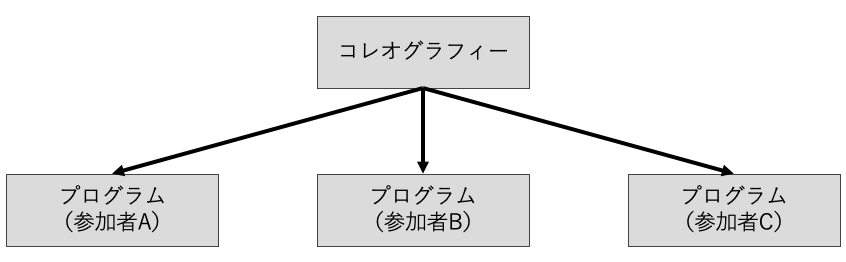
\includegraphics[scale=0.3]{image/epp.png}
  \caption{エンドポイント射影(参加者3人)}
\end{figure}
\vspace*{-15pt}
%%%%%%%%%%%%%%%%%%%%%%%%%%%%%%
%\section{Mypy}
%%Pythonは動的型付け言語で実行時にのみエラーが表示される.
%MypyはPythonの静的型検査器である.
%%Pythonは動的型付け言語で実行時にのみエラーが表示されるが,Mypyによる型注釈を活用することで
%%コンパイル時にバグの検出が可能になり,安全なコーディングが可能となる.
%%これによりコンパイル時にバグの検出が可能になり,安全なコーディングが可能となる.
%本研究ではMypyを別のPythonアプリケーションに統合するために,PythonプログラムにMypy.apiをインポートして型検査を行う.
%図\ref{mypyproc}は通常のMypyを使用した際の型検査のプロセスである.
%\begin{figure}[H]
%  \centering
%  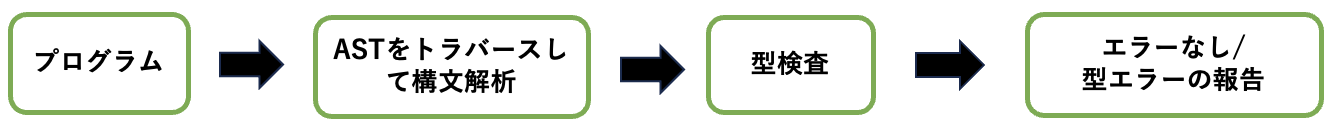
\includegraphics[scale=0.36]{image/mypyprocess.png}
%  \caption{Mypyプロセス}
%  \label{mypyproc}
%\end{figure}
%\vspace*{-20pt}
%%%%%%%%%%%%%%%%%%%%%%%%%%%%%%
\section{PyChoral}

PyChoralはPythonベースのコレオグラフィックプログラミング言語である.
Pythonは動的型付け言語であるため,Pythonの静的型検査器であるMypyを使用してコンパイル時に型検査を行う.
PyChoralでコレオグラフィを記述し,コンパイル時に各参加者のPythonプログラムがコレオグラフィに従った形で自動導出する.
code\ref{ch}はPyChoralプログラムの例である.
\vspace{-10pt}
\begin{lstlisting}[caption=Staff(S)とCustomer(C)でのお会計時のやり取り,label=ch]
class Check(Ch2[S,C]):
  def __init__(self):
    self.ch_CS:Channel[int,C,S] = Channel[int,C,S]('C','S')
    self.ch_SC:Channel[str,S,C] = Channel[str,S,C]('S','C')
  def check(self,price:At[int,S],money:At[int,C]) -> At[str,C]:
    payment = self.ch_CS.com(money)
    if (payment > price):
      return self.ch_SC.com("thanks"@S())
    else:
      return self.ch_SC.com("not enough"@S())
\end{lstlisting}
クラス\textsf{Check}の引数である\textsf{Ch2[S,C]}は,参加者S,Cがこのクラスに関連することを表す.
\textsf{Channel}は第1引数に通信する値の型,第2,3引数にそれぞれ送信者、受信者の型をもつ型クラスである.
\textsf{At}は第1引数に値の型,第2引数にその値に関連する参加者の型をもつ型クラスである.
\textsf{e@R()}は参加者Rの値eであることを示す.
\textsf{com}は送信者の値を受信者に転送するメソッドである.%($\texttt{At[\_,R1]} \rightarrow \texttt{At[\_,R2]}$).
%このPyChoralで記述したコレオグラフィより各参加者(S,C)のPythonプログラムを自動導出する.
%\begin{lstlisting}[caption=生成されたPythonプログラム]
%# Customer
%class Check_C():
%  def __init__(self):
%    self.ch_CS = Channel[int,C,S]()
%    self.ch_SC = Channel[str,S,C]()
%  def check(self):
%    Unit.id(self.ch_CS.com(1000))
%    return self.ch_SC.com()
%# Staff
%class Check_S():
%  def __init__(self):
%    self.ch_CS = Channel[int,C,S]()
%    self.ch_SC = Channel[str,S,C]()
%  def check(self,price):
%    payment = self.ch_CS.com()
%    if payment>price:
%      return Unit.id(self.ch_SC.com("thanks"))
%    else:
%      return Unit.id(self.ch_SC.com("not enough"))
%\end{lstlisting}

PyChoralは図\ref{pychoralprocess}のように,一度型検査を行なった後に各エンドポイントのASTを再構築し,各エンドポイントのPythonプログラムを生成する.
\vspace{-7pt}
\begin{figure}[H]
  \centering
  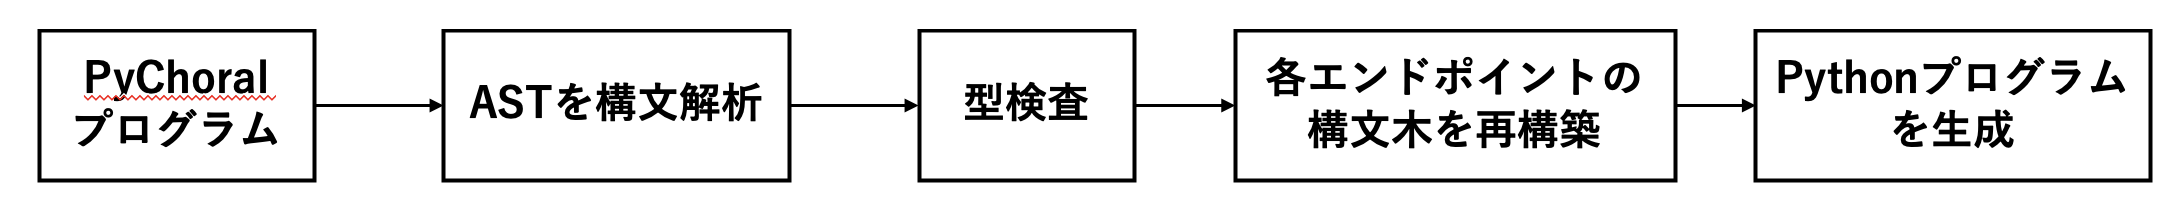
\includegraphics[scale=0.23]{image/pychoralprocess.png}
  \caption{PyChoralプロセス}
  \label{pychoralprocess}
\end{figure}
\vspace{-17pt}
\subsection{PyChoralの仕様}
図\ref{syntax}はPyChoralの構文のうち,既存のPythonとの差分がある部分である.
クラス定義は,参加者の明示をするためにChクラスを追加し,これを第一引数にとるものとする.
関数定義は,引数(self以外)に型注釈をつけることで関連する参加者を示す.式はリテラルのみ$\mblue{@}$をつけて参加者の情報を得る.
その他の式や文は型注釈もしくはMypyによる型検査の際に取得できる型情報から参加者の情報を得る.
\vspace{-8pt}
\begin{figure}[H]
  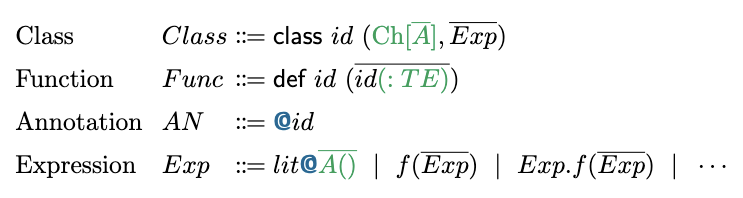
\includegraphics[scale=0.67]{image/diffpy.png}
  \caption{PyChoralの構文(一部)}
  \label{syntax}
\end{figure}
\vspace{-20pt}
とあるコレオグラフィの参加者$\cyan{\text{A}}$に対するPyChoralの項の射影は$\projection{Term}{A}$と記し,これは$Term$における参加者$\cyan{\text{A}}$の振舞いを表すPythonの項となる.
例えば,クラス定義の射影はクラス継承の第一引数Chクラスに存在する参加者名によってPythonの項を生成する.
\begin{alignat*}{2} 
  &\projection{\textsf{class} ~id~(Ch[\overline{\cyan{R}}],\overline{Exp}):\overline{Stm}}{A}=\\
  &
  ~~~~~~~~~~~~~~\begin{cases}
    \textsf{class} ~id\_{\cyan{A}}~(\overline{\projection{Exp}{A}}):\overline{\projection{Stm}{A}} & \text{if}~~ {\cyan{A}} \in \overline{\cyan{R}}\\
    \text{absent} & \text{if}~~ {\cyan{A}} \notin \overline{\cyan{R}}\\
  \end{cases}
\end{alignat*}
%例えば,代入文は以下のように定義される.
%\begin{alignat*}{2} 
%  & \projection{id:\tau = Exp}{A} =
%  \begin{cases}
%    id = \projection{Exp}{A} & \text{if}~ {\color{cyan}A} \in \text{rolesOf\_t}(\tau)\\
%    \projection{Exp}{A} & \text{otherwise}
%  \end{cases}\\
%\end{alignat*}
%\textsf{rolesOf\_t}は型$\tau$から参加者の型を文字列として返す関数である.$\projection{Exp}{A}$で式は再帰的に射影されて,文字列となる.
%
%(例) $\text{A} \rightarrow \text{B}$へのメッセージ
(例)参加者$\cyan{\text{A}},\cyan{\text{B}}$が関わるクラス$\textsf{Foo}$の射影
\begin{alignat*}{2} 
  &~~~~~~~~~\textsf{PyChoral} ~~~~~~~~~~~\Rightarrow~~~~ \textsf{Python}\\
  &\projection{\textsf{class} ~\text{Foo} \text{(Ch2[{\cyan{A}},{\cyan{B}}])}}{A} ~\Rightarrow~ \textsf{class} ~\text{Foo\_{\cyan{A}}}(~)\\
  &\projection{\textsf{class} ~\text{Foo} \text{(Ch2[{\cyan{A}},{\cyan{B}}])}}{B} ~\Rightarrow~ \textsf{class} ~\text{Foo\_{\cyan{B}}}(~)\\
  &\projection{\textsf{class} ~\text{Foo} \text{(Ch2[{\cyan{A}},{\cyan{B}}])}}{C} ~\Rightarrow~ 
\end{alignat*}
\subsection{エンドポイント射影の実装}
本研究では既存のPythonパーサーを活用する.Choralでは\mblue{@R}を各インターフェースに付属させることで参加者の情報を取得していたが,
Mypyの検査器は\mblue{@}を認識できないため,その際に参照する標準ライブラリ\textsf{typeshed}内のファイルにAtクラス,Channelクラスを追加し,
参加者の情報を取る.Importを含む文,ブロック,クラス定義,関数定義は射影後に独自のデータ構造で生成される.
親クラス\textsf{Stmt}は抽象的な構文木であり,クラス継承を使ってASTの具体的なノードを子クラス(\textsf{Block,ClassDef,...})として定義している.
新しく定義したデータクラスはMypyに備わっている標準のデータクラスから射影定義に従って必要なパラメータのみ抽出したものである.
\begin{lstlisting}[caption=data.py,label=data]
class Stmt:
    pass
class Block(Stmt): # list[stm]
    def __init__(self, body:list[Stmt]):
        self.body = body
... 
\end{lstlisting}
PyChoralプログラムの射影は\textsf{projection.py}に定義している.\textsf{projection}はStatementのリスト\textsf{n},
射影される参加者\textsf{r},型検査器\textsf{tc}を引数にとり,新しいデータ構造を返す関数である.\textsf{n}の要素\textsf{node}
に対して$\textsf{isinstance()}$で型を制限し,それぞれの射影関数に渡す.

\begin{lstlisting}[caption=projection.py,label=data]
def projection_all(n:list[Statement],r:str,tc:TypeChecker) -> list[Stmt]:
  result:list[Stmt] = [ ]
  for node in n:
      if isinstance(node,Import):
          result += [projection_md(node)]
      elif isinstance(node,ClassDef):
          result += [projection_class(node,r,tc)]
      ...
  return result
\end{lstlisting}
\subsection{アプリケーションによる評価}
%以下はPyChoralでのMergeSortの実装プログラムである.
%PyChoralを用いたアプリケーションとしてMergeSortを実装し,PyChoralの有用性を確認した。

%%%%%%%%%%%%%%%%%%%%%%%%%%%%%%%%%
\section{結論}
本研究はPythonを拡張したコレオグラフィックプログラミング言語PyChoralを実装した.PyChoralプログラムは射影の定義によって各参加者のPythonプログラムが生成される.
これらはコレオグラフィに従っているため,デッドロック等の並行性起因エラーが生じないことが保証されている.これにより,マルチスレッド環境におけるプログラムが
単一の言語で記述されるプログラムによって実装可能となり,Pythonプログラマの手助けとなる.3者間までの通信しか対応していないため,それ以上の参加者に対応可能にすることが今後の課題である.
%%%%%%%%%%%%%%%%%%%%%%%%%%%%%%%%%
%参考文献
\bibliography{reference_resume.bib}

\end{document}